% @author Huyen Tran, Claudia Porto DONE
\label{matrix-perfect-matching}
Marcin Mucha and Piotr Sankowski introduced new methods for finding perfect matching for both general and bipartite graphs which are based on randomization. The running time of these methods is $O(n^\omega)$, where $\omega$ is the smallest number such that two n×n matrices can be multiplied together. The current best-known value of $\omega$ is less than 2.38. These methods are easy to implement in $O(n^3)$ time, with the only tricky part being the fast matrix multiplication. \cite{Mucha-Sankowski}.

\subsubsection*{Matchings, Adjacency Matrices, and Their Inverses}
The method uses the mathematical framework that connects graph theory and linear algebra, focusing on matchings in graphs and their representation through adjacency matrices. By examining skew symmetric adjacency matrices and their properties, we can gain insights into the existence and identification of perfect matchings. This exploration also includes the development of algorithms, both randomized and deterministic, to efficiently determine matchings in bipartite graphs.

\paragraph*{Skew Symmetric Adjacency Matrix:} A matrix \( A \) is skew symmetric if \( A^T = -A \), meaning the transpose of \( A \) is equal to the negative of \( A \). The transpose of a matrix refers to the operation of flipping the matrix over its diagonal, so the rows of the original matrix become the columns in the transposed matrix, and vice versa. 
\noindent For a given graph \( G = (V, E) \), a skew-symmetric adjacency matrix \( \tilde{A}(G) \) is constructed with entries defined as:
\[
\tilde{A}_{i,j}(G) =
\begin{cases} 
x_{i,j} & \text{if } (v_i, v_j) \in E \text{ and } i < j, \\
-x_{i,j} & \text{if } (v_i, v_j) \in E \text{ and } i > j, \\
0 & \text{otherwise}.
\end{cases}
\]
Here, $x_{i,j}$ are unique variables assigned to edges in $E$. According to Tutte's theorem, the symbolic determinant \( \det \tilde{A}(G) \) is non-zero if and only if $G$ has a perfect matching.

\noindent To determine a perfect matching, unique random values are substituted for the symbolic variables, resulting in a random adjacency matrix \( A(G) \). By the Schwartz-Zippel lemma, with high probability, \( \det A(G) \neq 0 \) indicates the presence of a perfect matching. This leads to a randomized algorithm for determining if a graph has a perfect matching by computing the determinant of $A(G)$. The same method applies to bipartite graphs, where the symbolic determinant of the bipartite adjacency matrix is non-zero if the graph has a perfect matching. This can be done in $O(n^\omega)$ time using fast matrix multiplication. 

\noindent For example, given a graph $G=(V,E)$ with \( U = \{ u_1, u_2, u_3 \} \) and \( V = \{ v_1, v_2, v_3 \} \) and \\
$E=\{(v1,u1), (v1,u3), (v2,u1), (v3,u2), (v3,u3)\}$ represented in Figure \ref{fig:pm graph} , we can generate a the skew-symmetric adjacency matrix and then assign random value for each edge as in Figure \ref{fig:matrices}
\begin{figure}[h!]
\centering
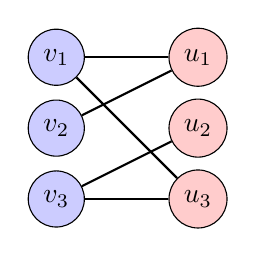
\begin{tikzpicture}[scale=0.9, every node/.style={circle, draw, minimum size=0.4cm}]
    % Define coordinates for the left (V) and right (U) sets
    \node[fill=blue!20] (v1) at (0, 2) {$v_1$};
    \node[fill=blue!20] (v2) at (0, 1) {$v_2$};
    \node[fill=blue!20] (v3) at (0, 0) {$v_3$};
    
    \node[fill=red!20] (u1) at (2, 2) {$u_1$};
    \node[fill=red!20] (u2) at (2, 1) {$u_2$};
    \node[fill=red!20] (u3) at (2, 0) {$u_3$};
    
    % Draw edges between the sets
    \draw[thick] (v1) -- (u1);
    \draw[thick] (v1) -- (u3);
    \draw[thick] (v2) -- (u1);
    \draw[thick] (v3) -- (u2);
    \draw[thick] (v3) -- (u3);
\end{tikzpicture}
\caption{Representation of graph $G=(V,E)$ with \( U = \{ u_1, u_2, u_3 \} \) and \( V = \{ v_1, v_2, v_3 \} \) and
$E=\{(v1,u1), (v1,u3), (v2,u1), (v3,u2), (v3,u3)\}$.}
\label{fig:pm graph}
\end{figure}

\begin{figure}[h]
    \centering
    % First matrix (a)
    \begin{subfigure}[b]{0.4\textwidth}
        \centering
        \[
        \tilde{A}(G) =
        \begin{bmatrix}
        0 & 0 & 0 & x_{1,1} & 0 & x_{1,3} \\
        0 & 0 & 0 & -x_{2,1} & 0 & 0 \\
        0 & 0 & 0 & 0 & -x_{3,2} & x_{3,3} \\
        -x{1,1} & -x_{2,1} & 0 & 0 & x_{4,5} & 0 \\
        0 & 0 & x_{3,2} & 0 & 0 & 0 \\
        -x_{1,3} & 0 & -x_{3,3} & 0 & 0 & 0
        \end{bmatrix}
        \]
        \caption{Symbolic skew-symmetric adjacency matrix (a).}
    \end{subfigure}
    \hfill
    % Second matrix (b)
    \begin{subfigure}[b]{0.4\textwidth}
        \centering
        \[
        \tilde{A}(G) =
        \begin{bmatrix}
        0 & 0 & 0 & 3 & 0 & 7 \\
        0 & 0 & 0 & -5 & 0 & 0 \\
        0 & 0 & 0 & 0 & -8 & 4 \\
        -3 & 5 & 0 & 0 & 0 & 0 \\
        0 & 0 & 8 & 0 & 0 & 0 \\
        -7 & 0 & -4 & 0 & 0 & 0
        \end{bmatrix}
        \]
        \caption{Randomized adjacency matrix with assigned weights (b).}
    \end{subfigure}
    \caption{Comparison of the symbolic skew-symmetric adjacency matrix (a) and the randomized adjacency matrix (b).}
    \label{fig:matrices}
\end{figure}

\paragraph*{Matrix Rank and Maximum Matching:}
Lovasz extended the approach by showing that the rank of \( A(G) \) equals twice the size of the maximum matching in \( G \) with high probability. This forms the basis for algorithms that compute the determinant or rank of \( A(G) \) using randomized substitutions and fast matrix operations. For example, \( O(n^\omega) \) time complexity is achieved for determinant computation, where \( \omega \) is the matrix multiplication exponent, currently \( \omega < 2.38 \).

\paragraph*{Allowed Edges:}
To construct a perfect matching, the algorithm identifies \textbf{allowed edges}, edges guaranteed to belong to some perfect matching. Using matrix inversion, Rabin and Vazirani showed that the inverse matrix \( A^{-1}(G) \) provides edge information: if \( (v_i, v_j) \in E \), then \( A^{-1}_{j,i} \neq 0 \) implies that \( (v_i, v_j) \) is an allowed edge.

\noindent The algorithm iteratively identifies an allowed edge, removes its endpoints from \( G \), and updates the adjacency matrix \( A(G') \) for the reduced graph \( G' \). By employing Gaussian elimination techniques and leveraging the Schur complement, the matrix updates are performed efficiently to avoid recomputation, maintaining an \( O(n^\omega) \) runtime.


\subsubsection{Constructing Matchings via Gaussian Elimination} 
The construction of matchings uses Gaussian elimination to systematically reduce the adjacency matrix of the graph while preserving information about perfect matchings. This process ensures computational efficiency and avoids recomputing matrices from scratch.

\paragraph*{Schur Complement and Matrix Update:}
Given a random adjacency matrix \( A(G) \) of a bipartite graph \( G = (U, V, E) \), let \( A^{-1}(G) \) be its inverse. If an edge \( (u_1, v_1) \in E \) satisfies \( A^{-1}_{1,1} \neq 0 \), then \( (u_1, v_1) \) is an \textbf{allowed edge} and can be chosen as part of the matching. However, recomputing \( A^{-1}(G) \) for the reduced graph \( G' = G - \{u_1, v_1\} \) from scratch would result in an \( O(n^{\omega+1}) \) algorithm. Instead, the Elimination Theorem states that the inverse of a submatrix can be updated using the Schur complement. The Schur complement is a derived matrix that provides a more efficient update mechanism.\\
Given a block matrix:
\[
A = \begin{bmatrix}
A_{11} & A_{12} \\
A_{21} & A_{22}
\end{bmatrix}
\]
where \(A_{11}\) and \(A_{22}\) are square matrices, the Schur complement of \(A_{22}\) in \(A\) is defined as:
\[
S = A_{11} - A_{12} A_{22}^{-1} A_{21}
\]
The Schur complement \(S\) is used to update the inverse of the submatrix \(A_{11}\) when \(A_{22}\) is inverted. This is particularly useful in the context of Gaussian elimination.\\
Therefore, when 
\[
A = 
\begin{bmatrix}
a_{1,1} & \mathbf{v}^T \\
\mathbf{u} & B
\end{bmatrix},
\quad
A^{-1} = 
\begin{bmatrix}
\hat{a}_{1,1} & \hat{\mathbf{v}}^T \\
\hat{\mathbf{u}} & \hat{B}
\end{bmatrix},
\]
\[
\text{where } \hat{a}_{1,1} \neq 0. \text{ Then } B^{-1} = \hat{B} - \frac{\hat{\mathbf{u}} \hat{\mathbf{v}}^T}{\hat{a}_{1,1}}.
\]

\noindent This result enables an efficient \( O(n^3) \) algorithm for finding perfect matchings using iterative updates without recomputation of the full matrix.

\paragraph*{Simple Algorithms for Perfect Matchings:}
Using Gaussian elimination, the following algorithms for perfect matching are defined:
\begin{enumerate}
    \item \textbf{Bipartite Graphs:} For bipartite graphs, the algorithm iteratively eliminates rows and columns corresponding to matched vertices while maintaining the inverse of the updated matrix. Allowed edges are identified by non-zero entries in \( A^{-1} \).
    \item \textbf{General Graphs:} For general graphs, additional elimination steps ensure symmetry in row and column updates. The process guarantees that allowed edges are correctly preserved.
\end{enumerate}

The algorithms for perfect matchings follow this general structure:
\begin{algorithm}
\caption{Simple algorithm for perfect matchings in bipartite graphs}
\textsc{Simple-Bipartite-Matching}($G$):
\begin{algorithmic}[1]
    \STATE $B = A^{-1}(G)$
    \STATE $M = \emptyset$
    \FOR{$c = 1$ to $n$}
        \STATE find a row $r$, not yet eliminated, and such that $B_{r,c} \neq 0$ and $A(G)_{c,r} \neq 0$ (i.e. $(u_c, v_r)$ is an allowed edge in $G - V(M)$)
        \STATE eliminate the $r$-th row and the $c$-th column of $B$
        \STATE add $(u_c, v_r)$ to $M$
    \ENDFOR
\end{algorithmic}
\end{algorithm}

Both algorithms achieve \( O(n^3) \) complexity due to efficient elimination and matrix inversion techniques.

\noindent \textbf{Example of Simple Bipartite Matching:} Given the graph $G=(E,V)$ in Figure \ref{fig:pm graph}, with the skew-symmetric adjacency matrix $A(G)$ in Figure \ref{fig:matrices}. Since the adjacency matrix \( A(G) \) can be represented as a block matrix:
\[
A(G) = 
\begin{bmatrix}
0 & A_{12} \\
A_{21} & 0
\end{bmatrix},
\]
where \( A_{12} \) corresponds to the edges from \( V \) to \( U \), and \( A_{21} = -A_{12}^T \) because $G$ is a bipartite graph. The matrix \( A_{12} \) is given by:
\[
A_{12} =
\begin{bmatrix}
3 & 0 & 7 \\
-5 & 0 & 0 \\
0 & -8 & 4
\end{bmatrix}.
\]
We can find the perfect matching in $G$ using the \textit{Simple-Bipartite-Matching} algorithm as follows:\\
\textbf{Initialization.} We compute the inverse of \( A = A_{12} \), denoted as \( B = A^{-1} \), which will be used to trace through the algorithm. For this example:
\[
\renewcommand{\arraystretch}{1.5}
B =
\begin{bmatrix}
0 & -\frac{1}{5} & 0 \\
\frac{1}{14} & \frac{3}{70} & -\frac{1}{8} \\
\frac{1}{7} & \frac{3}{35} & 0
\end{bmatrix}.
\]

\textbf{$c=1$: } Pick edge \( (v_2, u_1) \). Because \( B_{2,1} = \frac{1}{14} \neq 0 \) and \(A_{12} = -5 \neq 0 \) , which makes it valid. Therefore, add \( (v_2, u_1) \) to the matching and remove \( v_2 \) and \( u_1 \) from the graph, and update \( B \):
\[
\renewcommand{\arraystretch}{1.5}
B =
\begin{bmatrix}
0 & -\frac{1}{5} & 0 \\
0 & 0 & 0 \\
\frac{13}{98} & \frac{39}{490} & \frac{1}{56}
\end{bmatrix}.
\]

\textbf{$c=2$: } Pick edge \( (v_3, u_2) \). Because \( B_{3,2} = \frac{39}{490} \neq 0 \) and \(A_{12} = -8 \neq 0 \) , which makes it valid. Therefore, add \( (v_3, u_2) \) to the matching, remove \( v_3 \) and \( u_2 \) from the graph, and update \( B \):
\[
\renewcommand{\arraystretch}{1.5}
B =
\begin{bmatrix}
\frac{13}{195} & -\frac{117}{650} & \frac{1}{28} \\
0 & 0 & 0 \\
-\frac{13}{49} & -\frac{117}{163} & 0
\end{bmatrix}.
\]

\textbf{$c=3$: } Pick edge \( (v_1, u_3) \). Because \( B_{1,3} = \frac{1}{28} \neq 0 \) and \(A_{12} = 7 \neq 0 \) , which makes it valid. Therefore, add \( (v_1, u_3) \) to the matching and remove \( v_1 \) and \( u_3 \) from the graph, and update \( B \):
\[
\renewcommand{\arraystretch}{1.5}
B =
\begin{bmatrix}
0 & 0 & 0 \\
0 & 0 & 0 \\
-\frac{13}{49} & -\frac{117}{163} & 0
\end{bmatrix}.
\]

\textbf{Result:} The final perfect matching is: $M = \{(v_1, u_3), (v_2, u_1), (v_3, u_2)\}.$


\paragraph*{Matching Verification and Lazy Elimination:}
To verify matchings and find maximal allowed submatchings, a simplified version of Gaussian elimination, called \textbf{lazy elimination}, is employed. Instead of updating all matrix elements immediately, changes are accumulated in compact forms, such as \( \mathbf{u} \mathbf{v}^T / c \), and applied in batches during critical steps. This approach allows verification of inclusion-wise maximal matchings in \( O(n^\omega) \) time.

\begin{algorithm}
\caption{Gaussian elimination with no pivoting}
\textsc{Simple-Elimination}($X$):
\begin{algorithmic}[1]
    \FOR{$i = 1$ to $n$}
        \STATE lazily eliminate the $i$-th row and $i$-th column of $X$;
        \STATE let $j$ be the largest integer such that $2^j \mid i$;
        \STATE \textbf{UPDATE}($\{i + 1, \ldots, i + 2^j\}, \{i + 1, \ldots, n\}$);
        \STATE \textbf{UPDATE}($\{i + 2^j + 1, \ldots, n\}, \{i + 1, i + 2^j\}$);
    \ENDFOR
\end{algorithmic}
\end{algorithm}

\textbf{Example of Gaussian Elimination with No Pivoting}

Consider the following matrix $A(G)$:
\[
A(G) = 
\begin{bmatrix} 
1 & 0 & 1 \\
1 & 1 & 0 \\
0 & 1 & 1
\end{bmatrix}
\]

\begin{enumerate} 
\item \textbf{Eliminate the first row and column:} 
    \begin{itemize}
        \item The first element \( A_{1,1} = 1 \) is already non-zero
         \item Subtract the first row from the second row to eliminate the first column in the second row:
        \[
        \begin{bmatrix} 
        1 & 0 & 1 \\
        0 & 1 & -1 \\
        0 & 1 & 1
        \end{bmatrix}
        \]
        \item Subtract the first row from the third row to eliminate the first column in the third row:
        \[
        \begin{bmatrix} 
        1 & 0 & 1 \\
        0 & 1 & -1 \\
        0 & 1 & 1
        \end{bmatrix}
        \]
    \end{itemize}

\item \textbf{Eliminate the second row and column:}
    \begin{itemize}
        \item The second element \( A_{2,2} = 1 \) is non-zero.
        \item Subtract the second row from the third row to eliminate the second column in the third row:
        \[
        \begin{bmatrix} 
        1 & 0 & 1 \\
        0 & 1 & -1 \\
        0 & 0 & 2
        \end{bmatrix}
        \]
    \end{itemize} 

\item \textbf{Eliminate the third row and column:}
    \begin{itemize}
        \item The third element \( A_{3,3} = 2 \) is non-zero.
        \item No further elimination is needed as we have reached the last row.
    \end{itemize}
\end{enumerate}

The resulting upper triangular matrix is:
\[
U = 
\begin{bmatrix} 
1 & 0 & 1 \\
0 & 1 & -1 \\
0 & 0 & 2
\end{bmatrix}
\]

To find an inclusion-wise maximal allowed submatching, we can use the resulting upper triangular matrix \( U \). The non-zero entries in \( U \) indicate the allowed submatchings. In this case, the non-zero entries are:
\begin{itemize}
    \item \( U_{1,1} = 1 \)
    \item \( U_{2,2} = 1 \)
    \item \( U_{3,3} = 2 \)
\end{itemize}
These entries correspond to the inclusion-wise maximal allowed submatching.

\paragraph{Performance and Time Complexity}
The algorithm has a time complexity of $O(n^\omega)$, where $n$ is the number of vertices in the graph and $\omega$ is the matrix multiplication exponent (currently $\omega < 2.38$). The algorithm leverages randomized substitutions and efficient matrix operations, such as determinant computation and matrix inversion, to identify allowed edges and construct a perfect matching. While the algorithm is probabilistic (Monte Carlo), the error probability can be made arbitrarily small by choosing a sufficiently large finite field for the random substitutions. In practice, the algorithm is highly efficient for dense graphs, as its complexity depends on matrix multiplication rather than the number of edges.

\noindent Further details and implementation of this algorithm is discussed in Section \ref{pmReduction}
